\newpage
\subsection{[C] Sharing a list with a group}
In order to share a list with a group, hover on top of the bubble that represents the list and click on the gear icon.

% Inserire immagine delle opzioni che vengono fuori al passaggio del mouse sopra la bolla
\begin{figure}[H]
  \centering 
  
\includegraphics[scale=0.3]{Sections/3-HowToUse/Images/list_gear_icon.png}
  \caption{Button to show the available list's actions.}
\end{figure}

From the various options that are available, click on the one with the sharing icon.

% Inserire immagine dell'icona per condividere la lista
\begin{figure}[H]
  \centering 
  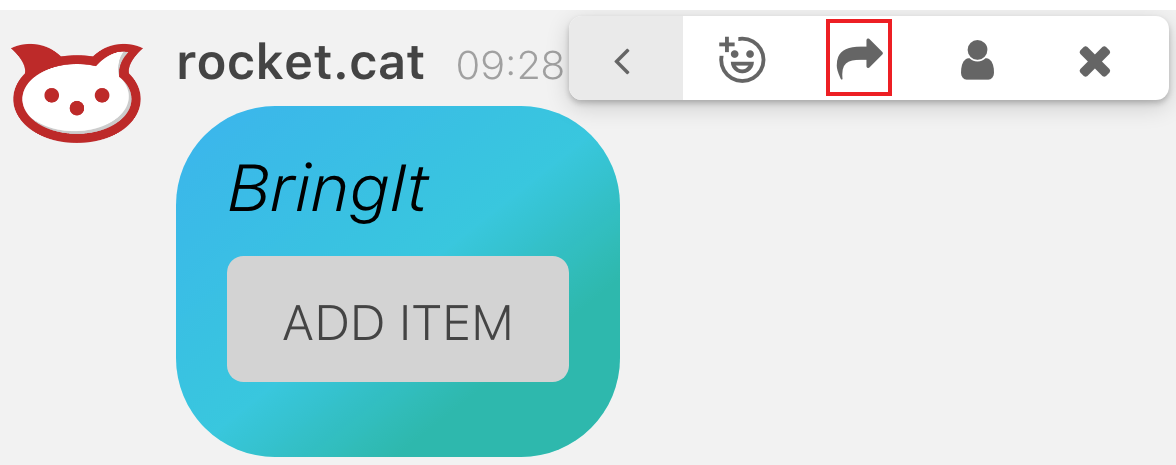
\includegraphics[scale=0.3]{Sections/3-HowToUse/Images/list_share_icon.png}
  \caption{Sharing button.}
\end{figure}

Once that the option has been clicked, the following popup will appear, showing the list of all the group that the list can be shared to.

% Inserire immagine del popup con la lista dei gruppi
\begin{figure}[H]
  \centering 
  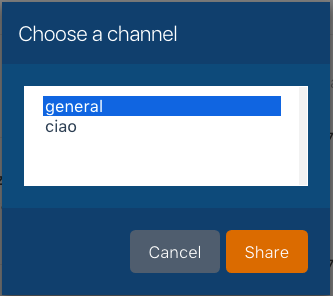
\includegraphics[scale=1.0]{Sections/3-HowToUse/Images/list_share_group.png}
  \caption{Popup showing the list of all the groups to which is possible sharing a list.}
\end{figure}

Now, select the group you want share the list with and then click on \textit{"Share"}. \\
This will open a new popup, letting you choose to which user you want to grant the \textbf{editor} permission. Once you have chose to which users to grant the permissions, click on \textit{"Ok"}.

% Immagine del popup con la lista degli utenti, alcuni selezionati
\begin{figure}[H]
  \centering 
  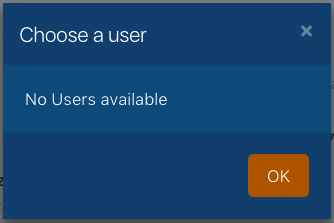
\includegraphics[scale=1.0]{Sections/3-HowToUse/Images/list_share_user.png}
  \caption{Popup to grant the editor permission to users inside the group.}
\end{figure}
